\section{System Design}
\label{section:system_design}

\subsection{High-Level Architecture}

\begin{figure}[H]
    \centering
    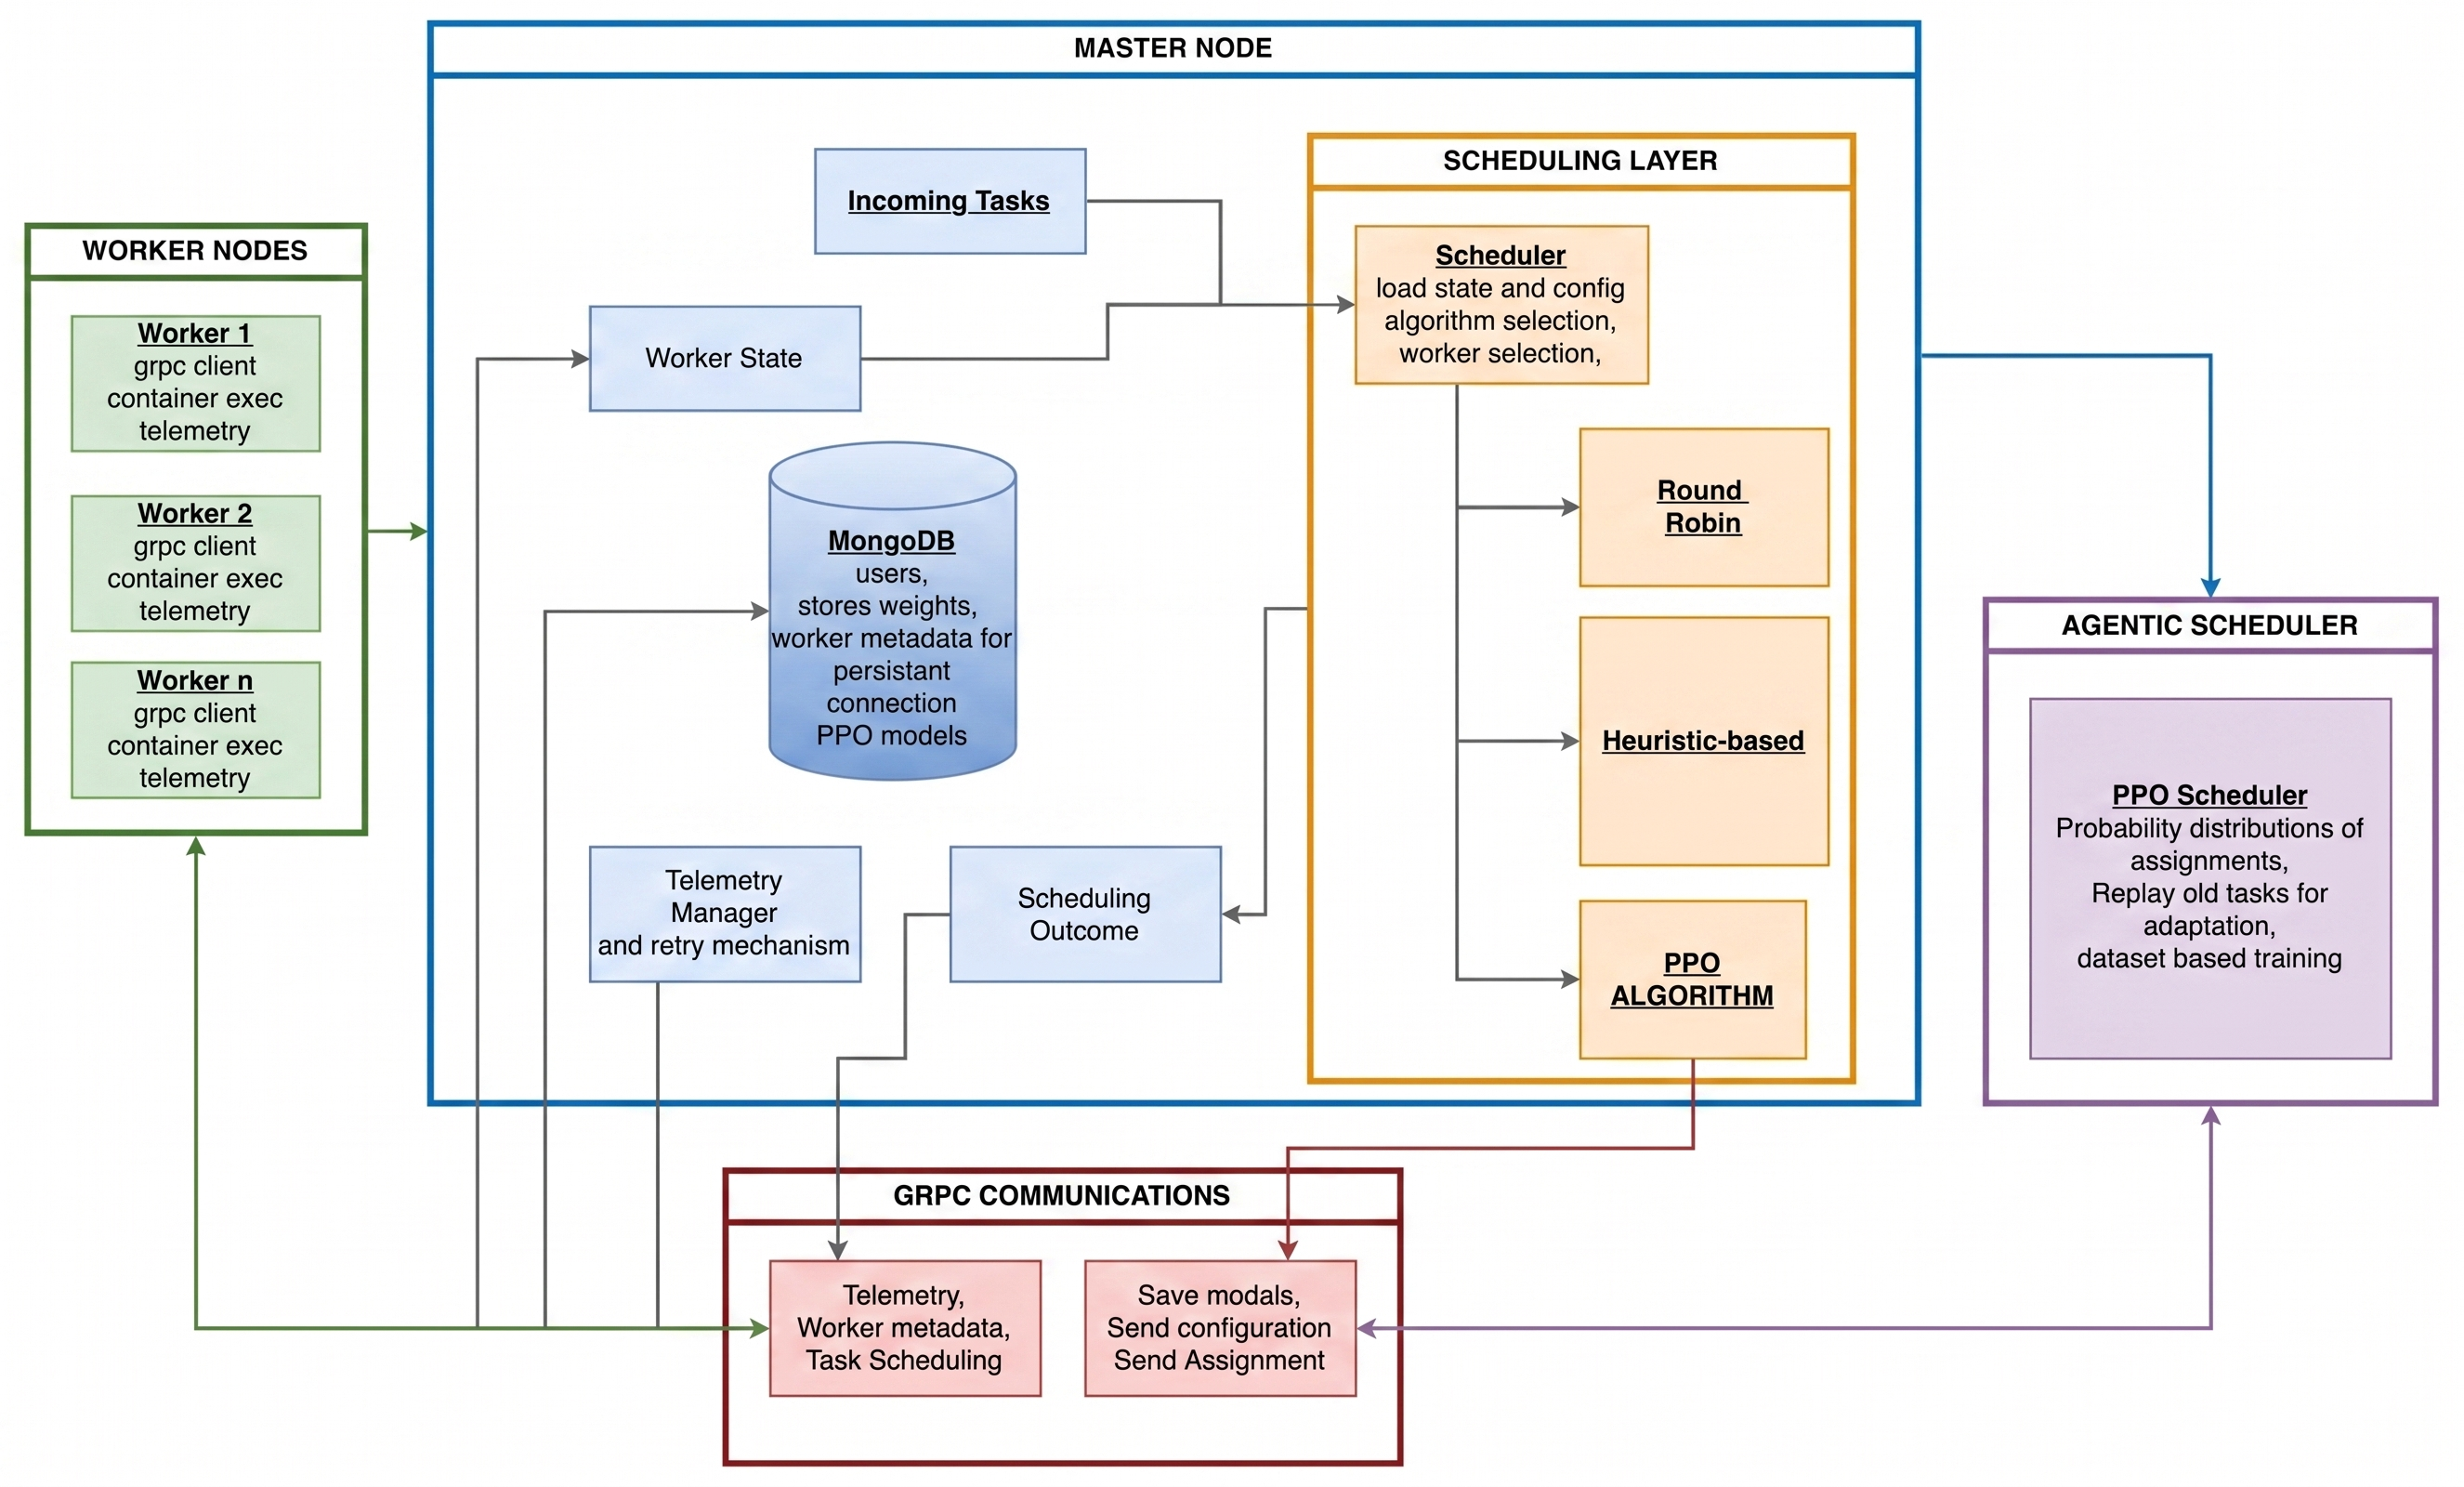
\includegraphics[width=\textwidth]{Figures/Architecture/overall_architecture_colored.png}
    \caption{Overall architecture of Agentic Cloud Cluster}
    \label{fig:overall_architecture}
\end{figure}

Description of Figure 1, the overall architecture: The system follows a master-worker layout. When a task comes in, the master node saves its details, keeps track of which workers are available, and asks the scheduler to choose one. The worker nodes then run the Docker containers they are given and send the results back to the master. Because the PPO scheduler runs as a separate Python service, the main Go control plane can stay stable on its own while the learning model is updated or retrained without affecting the rest of the system.

\subsection{Go Distributed Cluster Architecture}

The distributed cluster is achieved by a control plane in Go. Its design is based on a simple rule: the master decides to coordinate and the workers perform the work. This maintains the system easy to reason about. It is not necessary that a worker should know about other workers. It simply has to accept assignments of the master, execute the container and report health and task status.

At runtime, the cluster has four main layers:

\begin{enumerate}
    \item \textbf{Client and API layer}: this layer accepts a task submission and management commands.
    \item \textbf{Master control plane}: validates requests, stores task state, tracks workers, and picks a scheduler.
    \item \textbf{Scheduler layer}: selects a worker by Round-Robin, RTS or PPO.
    \item \textbf{Worker execution layer}: executes Docker containers and returns results.
\end{enumerate}

GRPC is used to communicate between master and workers. Request and response formats get declared in Protocol Buffer files, and makes communication rigid and typed. Persistent storage is also used by the master to store records of tasks, worker records, task attempt records and result metadata records. The design consideration here is that scheduling, execution, and persistence are independent modules. This facilitated easier debugging of the project since a scheduler bug would not necessitate the re-writing of the worker executor, and a bug in worker execution would not require the PPO model to be changed.

\subsection{Master Node}

The coordinator is the master node. Its responsibilities are:

\begin{itemize}
    \item Accept task submissions.
    \item Keep worker registry and worker health.
    \item Track available CPU, memory and storage.
    \item Invoke the active scheduler on each of the tasks.
    \item Assign workers to do tasks.
    \item Store task state, attempts and results.
    \item Requeue tasks in case of failure by workers or when resources are not available.
\end{itemize}

On the inside, the master has a couple of significant modules:

\begin{table}[H]
\centering
\caption{Master node modules}
\label{tab:master_modules}
\begin{tabularx}{\textwidth}{lX}
\toprule
\textbf{Module} & \textbf{Role} \\
\midrule
Server layer & Exposes gRPC calls being used by workers to register, heartbeat, task status, and report results. \\
Task handling & Generates tasks, records state transitions, queues tasks when workers are offline, and records attempts. \\
Registry of workers & Holds up-to-date worker identities, addresses, resource capacities, and current availability. \\
Scheduler package & Provides a common interface to Round-Robin, RTS, as well as PPO scheduling. \\
Persistence layer & Stores workers, tasks, assignments, attempts, and results. \\
Telemetry manager & Maintains the recent state of health and resources of workers to schedule and inspect the operators. \\
\bottomrule
\end{tabularx}
\end{table}

Of particular importance is the scheduler boundary. The master does not even have to be aware of the internal algorithm. It simply poses: given this task and these workers, which worker is to be given the task? The scheduler will reply with a worker ID and the master will verify that the worker has not disappeared yet and has sufficient resources before dispatching the task.

\subsection{Worker Node}

The worker node has the role of carrying out tasks. Every worker opens a gRPC server, accepts orders made by the master, launches a Docker container, monitors the execution, streams logs, and reports final status. The worker also transmits heartbeat information allowing the master to have a live view of cluster resources.

The worker is responsible of three things:

\begin{itemize}
    \item \textbf{Registration and heartbeat}: after registration, the worker periodically reports resource and status changes to the master.
    \item \textbf{Container execution}: the worker pulls or uses the requested Docker image, creates the container with the requested resource limits, runs it, and monitors the exit code.
    \item \textbf{Result reporting}: Once the container has left the worker reports success or failure and posts any output files produced by the task.
\end{itemize}

This makes the worker mostly stateless from a cluster point of view. When one worker unintentionally vanishes, the master will notice the missed heartbeats, and is also capable of requeuing tasks. The worker does not liaise with other workers, preventing the distributed locking of a complex nature.

\subsection{Control Flow in the Go Cluster}

Normal task flow is:

\begin{enumerate}
    \item A task is posted with image name, command and resource requirements.
    \item The master puts the task in created or queued state.
    \item The master develops a live picture of workable workers.
    \item The active scheduler picks a worker.
    \item The master articulates the task to such a worker using gRPC.
    \item The worker executes the Docker container and logs or streams logs.
    \item The worker gives a report on completion.
    \item The result is stored in the master which emancipates the worker resources.
\end{enumerate}

The system also promotes recovery behavior. In case a worker is lost, the master will record the attempt as lost and reenact the logical task. What is significant about this separation between a logical task and an attempt to execute the task is that a task may require many more than one attempt before it reaches a final state.

\subsection{Resource Accounting}

Resource accounting is concerned with scheduling. Every employee promotes a sum of the CPU, memory, and storage. The master tracks allow available resources to be tracked by the difference between the resources used by the tasks that are currently being assigned. As soon as a piece of work is done, these resources are freed. The simple types of schedulers use this accounting, as well as the action mask of PPO.

The design does not provide tasks to workers that they cannot fit in. Although PPO may be true about a worker, the Go master will still confirm the decision prior to assignment. This safeguards the cluster against stale model output or stale worker state.

\subsection{Task Lifecycle}

Tasks are first in the master queue and stay in the queue until at least one worker is available to meet the resource constraints. When feasible worker is available, the scheduler picks a target and the master picks an execution attempt. In case of dispatch failure because of stale state or connectivity failures, the attempt is marked lost and the logical task is returned to the queue to go through another scheduling cycle.

Once it has begun to execute, the worker sends back to the master status of completion. Complete runs are recorded as complete. Recoverable and non-recoverable: Failed runs are classified as recoverable or non-recoverable, recoverable failures are retried using requeueing, and non-recoverable failures terminate the task as failed.

\subsection{Task Execution Flow}

The definite path of execution begins at the API where the task is tested and stored and then transferred to the master queue. The queue processor constructs a new worker snapshot, calls the active scheduler, and checks the viability of the selected worker before reserving resources and sending an \texttt{AssignTask} call.

When the worker accepts and initiates the container, the effort is continued until the end and the master maintains the end result and releases reserved resources. In case of assignment or execution failure caused by transient failures (such as loss of workers), the attempt is marked lost and the logical task is requeued to reschedule it. It is this attempt-level recovery that allows safe retries without any loss in task-level traceability.

\subsection{Scheduler Interface}

The scheduler receives:

\begin{itemize}
    \item task CPU requirement,
    \item task memory requirement,
    \item store requirement,
    \item task type,
    \item worker capacity,
    \item worker availability,
    \item worker activity status.
\end{itemize}

It yields a worker ID. This easy interface enabled the project to begin with baselines and subsequently incorporate PPO. The PPO scheduler connects to a Python service using gRPC. When the PPO service is not available or has an inappropriate worker, the Go scheduler will revert to a safer scheduler. This was an intentional design choice since a learning model is expected to enhance scheduling, and not render the entire cluster vulnerable.

\subsection{PPO Deployment Design}

The PPO deployment is in support of three modes:

\begin{table}[H]
\centering
\caption{PPO deployment modes}
\label{tab:ppo_modes}
\begin{tabularx}{\textwidth}{lX}
\toprule
\textbf{Mode} & \textbf{Meaning} \\
\midrule
Active & PPO makes the scheduling decision and falls back on failure. \\
Shadow & PPO is queried for comparison, but the fallback scheduler is used for the actual placement. \\
Fallback & PPO is not used but the fallback scheduler is invoked directly. \\
\bottomrule
\end{tabularx}
\end{table}

This design was selected since the deployment of models in systems work should be conservative. The system is able to test the PPO decisions without necessarily believing them in the production paths.